\documentclass[tog]{acmsiggraph}

% fürs  code highlighting
\usepackage{listings}

% für hyperlinks http://en.wikibooks.org/wiki/LaTeX/Hyperlinks
\usepackage{hyperref}

% für korrkte Umlaute
\usepackage[utf8]{inputenc}

% für korrekte mathematische Zeichen
\usepackage{amsfonts}

% für deutschen Zeilenumbruch
\usepackage[ngerman]{babel}

% für Umlaute
\usepackage[T1]{fontenc}\usepackage{lmodern}

%%% Used by the ``review'' variation; the online ID will be printed on 
%%% every page of the content.

\TOGonlineid{45678}

%%% Used by the ``preprint'' variation.

\TOGvolume{0}
\TOGnumber{0}

\title{Digitale Bilder}

\author{Reguieg, Ibrahim Khaled\thanks{e-mail: Khaled.Reguieg@gmail.com}
\and Döring, Jules\thanks{e-mail: Jules.Doering@gmx.de}}
\pdfauthor{Reguieg, Döring}

\keywords{Digitale Bilder, Bildverarbeitung, CG1 }

\begin{document}

%%% This is the ``teaser'' command, which puts an figure, centered, below 
%%% the title and author information, and above the body of the content.

 \teaser{
   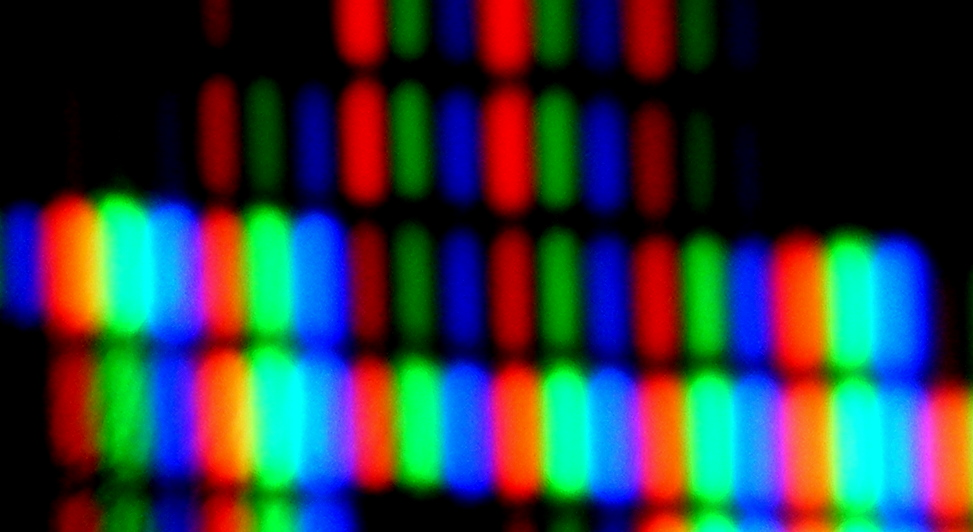
\includegraphics[width=7in, trim=10mm 10mm 8mm 60mm, clip=true]{images/Jeffrey_Smith_Flikr_CC-BY-ND-2-0.jpg}
   \caption{\href{https://www.flickr.com/photos/jmsmith000/3097202394}{Jeffrey Smith 2008 }}
 }

\maketitle



\section{Vorwort}
In der Realität werden Bilder durch reflektiertes Licht erzeugt.
Das führt zu den folgenden Fragestellungen:

"Wie stellen wir Farben und Bilder am Computer dar?"


"Wie werden Bilder im Computer repräsentiert?"

Hier soll ein Weg hergeleitet werden, diese in einer Form zu abstrahieren, mit der Computerprogramme effizient arbeiten können.
\end{abstract}

\section{Was ist ein Bild?}

\subsection{Mathematische Repräsentation:}
Am besten dafür eignet sich die folgende stetige mathematische Funktion,die die Menge der Koordinaten R auf die Menge der Farben V abbildet:
\begin{equation}I(x,y): R \rightarrow V\end{equation}
\begin{equation}R\subset \mathbb{R}^2\end{equation}
\begin{equation}V = \mathbb{R}^+ \: Graustufenbild\end{equation}
\begin{equation}V = \left (\mathbb{R}^+  \right )^3 \: Farbbild\end{equation}


Diese Art der Modellierung ist unnötig komplex. Da durch die biologischen Einschrängkungen denen die menschliche Wahrnehmung unterliegt einige Punkte wegfallen. Diese kann man zur Simplifizierung des Modells nutzen.
Zum Beispiel gilt: Je weiter ein Objekt entfernt ist, um so kleiner ist die Abbildung auf unserer Netzhaut. Da das Licht von verschiedenen Punkten des gesehenen Objekts auf den gleichen Punkt auf der Netzhaut projeziert wird. Somit hat das menschliche Auge keine Chance mehr die Unterschiede zwischen nahegelegenen Punkten wahrzunehmen.
Beim Druck findet dieses Begebenheit auch Anwendung, beispielsweise druckt der Druckkopf ganz kleine Muster, um aus Gelb und Magenta Rot oder Orange zu mischen.


\begin{figure}[ht]
  \centering
  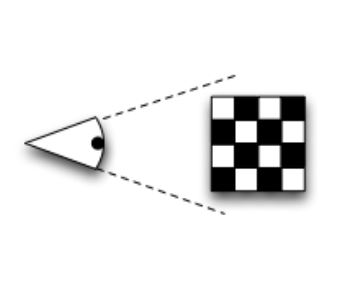
\includegraphics[width=0.75in]{images/AugeObjektNah}
  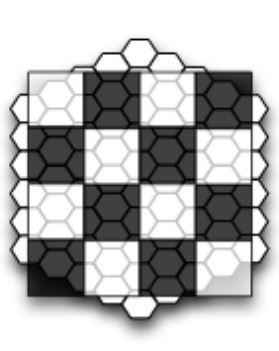
\includegraphics[width=0.5in]{images/SinneszelleObjektNah}
  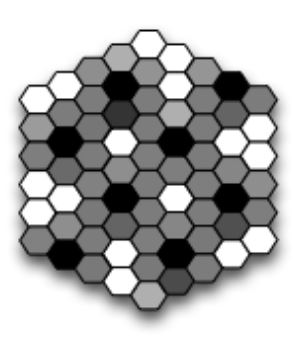
\includegraphics[width=0.5in]{images/AbbildungAufSinneszelleObjektNah}
  \caption{Objekt nah am Auge. 'Skript Rehfeld - Digitale Bilder'}
  \label{fig:Objekt nah am Auge}
\end{figure}

\begin{figure}[ht]
  \centering
  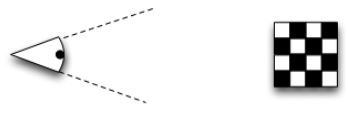
\includegraphics[width=1.5in]{images/AugeObjektFern}
  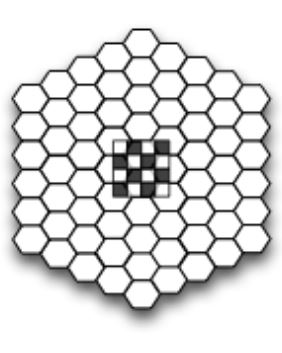
\includegraphics[width=0.5in]{images/SinneszelleObjektFern}
  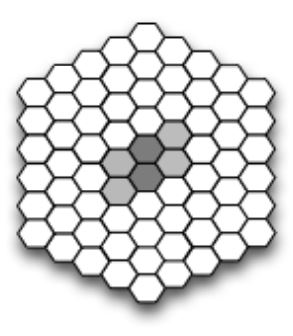
\includegraphics[width=0.55in]{images/AbbildungAufSinneszelleObjektFern}
  \caption{Objekt fern vom Auge. 'Skript Rehfeld - Digitale Bilder'}
  \label{fig:Objekt fern vom Auge}
\end{figure}

\begin{figure}[ht]
  \centering
  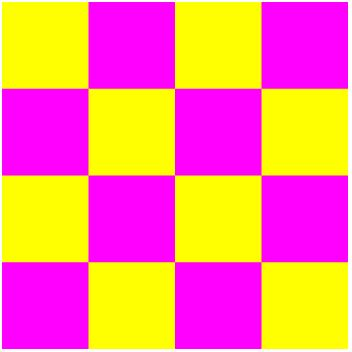
\includegraphics[width=0.5in]{images/gelbMagentaMusterGrob}
  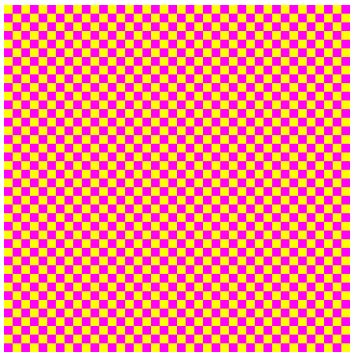
\includegraphics[width=0.5in]{images/gelbMagentaMusterFeiner}
  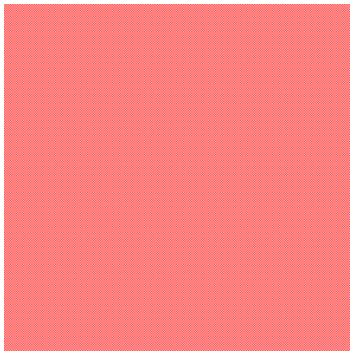
\includegraphics[width=0.5in]{images/gelbMagentaMusterFein}
  \caption{Farben mischen aus CMYK. 'Skript Rehfeld - Digitale Bilder'}
  \label{fig:Aus Grundfarben wird neue eine Farbe}
\end{figure}

Ähnlich verhält es sich bei Bildschirmen, denn die mangelnde örtliche Auflösung führt zum Eindruck eines stetigen Bildes, wobei die Signale des Bildschirms eigentlich diskret sind.

\section{Technische Umsetzung}
Die Modellierung des Bildgitters wird durch einen zweidimensionalen byte Array dargestellt.

Mithilfe dessen nun jeder Subpixel bearbeitet werden kann, indem wir mit zwei geschachtelten For-Schleifen über die Koordinaten iterieren und dort die RGB-Farbwerte setzen.
\begin{lstlisting}[language=Java]
final byte[][] pic = new byte [640][480][3];

for (int x = 0; x < width; ++x){
  for (int y = 0; y < height; ++y){
    byte r = pic [x][y][0];
    byte g = pic [x][y][1];
    byte b = pic [x][y][2];
    }
  }
\end{lstlisting}

Überlegungen in Hardware-naher Programmierung: Arrays sind quasi wie Pointer in C.

Der SRAM ist ein transistorbasierter Speicher, er bietet mehr Platz \rightarrow er\:ist\:teuer\:aber\:schnell

Der DRAM ist ein kondensatorbasierter Speicher, er bietet weniger Platz \rightarrow er\:ist\:günstig\:aber\:langsam

Deswegen befinden sich schnelle kleine Speicher auf der CPU die als  Caches benutzt werden.
Modernen CPUs haben üblicherweise drei Cache-Level mit denen man versucht die Cache Misses zu minimieren.

{\small\url{http://lwn.net/Articles/250967/}}


Die Modellierung eines Graustufenbildes geschieht als eindemensionales Array, um die Cacheprediction besser auszunutzen wird das Bild bzw. die Bildinformation zeilenweise hintereinander gelegt.

\begin{lstlisting}[language=Java]
final byte[][] pic = new byte [640 * 480];

for (int x = 0; x < width; ++x) {
	for (int y = 0; y < height; ++y) {
		byte g = pic [y * width +x];
	}
}
\end{lstlisting}

Die Modellierung eines Farbbildes geschieht als eindemensionales Array vom Typ Byte.
In diesen wird das Bild zeilenweise hintereinander gelegt und nach Farbkanälen getrennt.

\begin{lstlisting}[language=Java]
final byte[][] pic = new byte [640 * 480 * 3];
SomeImageLoader.loadInto(pic);
for (int x = 0; x < width; ++x) {
  for (int y = 0; y < height; ++y) {
	final byte red = pic[ 0 * width * 
		height + y * width + x ];

	final byte green = pic[ 1 * width * 
		height + y * width + x ];

	final byte blue = pic[ 2 * width * 
		height + y * width + x ];
    }
  }
\end{lstlisting}

bei der Modellierung eines Farbbildes als eindemensionales Array vom Typ Byte wird das Bild zeilenweise in je 3 aufeinander folgende Subpixel gestückelt und hintereinander gelegt.

\begin{lstlisting}[language=Java]
final byte[][] pic = new byte [640 * 480 * 3];

for (int x = 0; x < width; ++x){
  for (int y = 0 ; y < height; ++y){
    byte r = pic [y * width *3 + x*3 +0]; 
    byte g = pic [y * width *3 + x*3 +3];
    byte b = pic [y * width *3 + x*3 +2];
    }
  }
\end{lstlisting}

Die häufigste Darstellung ist allerdings die pixelweise Darstellung in einem Array vom Typ Integer.
Dabei sollte man das Prinzip des "Data structure alignment" beachten, das die Shiftoperationen ausnutzt, da sie der Arbeitsweise von CPU mit dem  Speicher ähnelt. Dies erhöht die Perfomanz. 


{\small\url{http://en.wikipedia.org/wiki/Data_structure_alignment}}


Bei der pixelweisen Darstellung in einem Array vom Typ Integer benutzt man Shiftoperationen und maskierrt die Speicherbereiche für den Zugriff auf die Subpixel. Das folgende Bild zeigt diese Struktur:

\begin{figure}[ht]
  \centering
  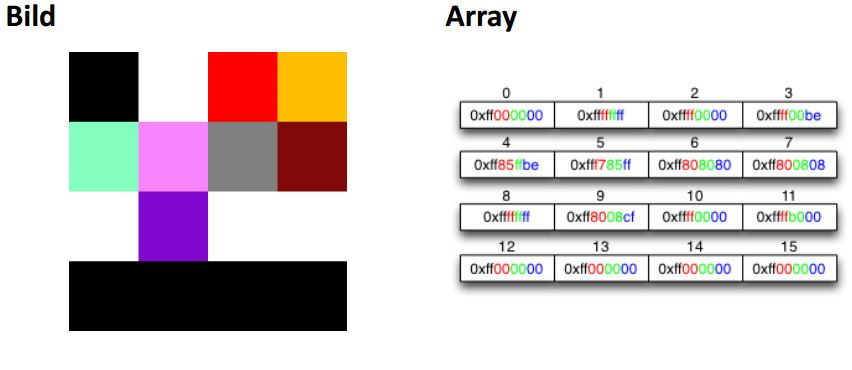
\includegraphics[width=2.0in]{images/BildPixelweiseInteger}
  \caption{Farbbild in pixelweiser Darstellung im Integer Array. 'Skript Rehfeld - Digitale Bilder'}
  \label{fig:Pixelweise Darstellung im Array.}
\end{figure}

\begin{lstlisting}[language=Java]
final int height = 480;
final int width = 640;
final int[] pic = new int[height * width ];
SomeImageLoader.loadInto( pic );
for( int y = 0; y < height; ++y ) {
	for( int x = 0; x < width; ++x ) {
	    int red = (pic[ y * width + x ] &
 	    0xff0000) >> 16;
	    int green = (pic[ y * width + x ] &
 	    0xff00) >> 8;
	    int blue = pic[ y * width + x ] & 0xff;

	    pic[y * width + x ] = 
	    ((red & 0xff) << 16) | 
	    ((green & 0xff) << 8) | 
	    (blue & 0xff);
	}
}
\end{lstlisting}



\section{Koordinatensystem}
Bei allen beschriebenen Vorgängen ist zu beachten, dass das in der Computergrafik übliche Koordinatensystem mathematisch korrekt unten links beginnt und sich nach oben und rechts ausbreitet.

\begin{figure}[ht]
  \centering
  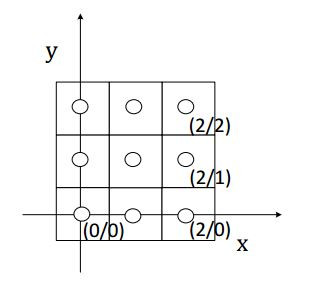
\includegraphics[width=1.0in]{images/koordinatenSystemComputergrafik}
  \caption{Bilder in der Computergrafik. 'Skript Rehfeld - Digitale Bilder'}
  \label{fig:Koordinatenursprung unten links}
\end{figure}

In der Bildverarbeitung hingegen beginnt es gemäß der Leserichtung der westlichen Kultur sowie der Richtung in CRT Monitoren, oben links und breitet sich nach rechts und unten aus.

\begin{figure}[ht]
  \centering
  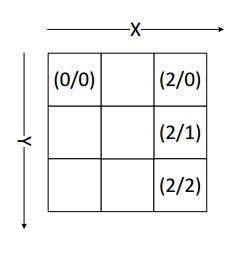
\includegraphics[width=1.0in]{images/koordinatenSystemBildverarbeitung}
  \caption{Bilder in der Bildverarbeitung. 'Skript Rehfeld - Digitale Bilder'}
  \label{fig:Koordinatenursprung oben links}
\end{figure}

\bibliographystyle{acmsiggraph}
\nocite{*}
\bibliography{template}
\end{document}

